\documentclass[11pt]{article}
\usepackage[a4paper,margin=2.3cm]{geometry}
\usepackage{amsmath}
\usepackage{graphicx}
\usepackage{booktabs}
\usepackage[hidelinks]{hyperref}
\usepackage{xurl}
\newcommand{\Msun}{\ensuremath{M_\odot}}
\newcommand{\Mpc}{\ensuremath{\,\mathrm{Mpc}}}

\title{LongChirp: an AI-assisted benchmark for searches of minutes-long\\ subsolar-mass inspirals in real LIGO noise}
\author{Sumit Pal\\ Independent researcher\\ ORCID \href{https://orcid.org/0009-0000-9541-2793}{0009-0000-9541-2793}}
\date{Draft, 28 November 2026}

\begin{document}
\maketitle

\begin{abstract}
On 1,344 simulated subsolar-mass binary inspirals added to real LIGO O3a data, a semi-coherent matched-filter bank
reaches a sensitive chirp distance of 57.5\Mpc{} at a false-alarm rate (FAR) of one per day and a convolutional neural
network (CNN) reaches 48.4\Mpc{}, about one third of the 155\Mpc{} reached by an ideal detector that knows each
signal's exact waveform and triggers at network signal-to-noise ratio (SNR) 8. We release this setting as
\emph{LongChirp}, a fixed benchmark for signals that stay in the detector band for minutes: 24 test and 8 development
segments of Hanford (H1) and Livingston (L1) strain from the Gravitational Wave Open Science Center, a committed
injection table, a 27.3-day time-slide background, and an evaluator that uses the submission format and found rule of
the first machine-learning gravitational-wave mock data challenge (MLGWSC-1). The bank leads the CNN in distance by a
factor 1.19 (90\% interval 1.10--1.29, resampling injections only) at one per day; under a $\pm1$\,s timing rule the
CNN reaches 25.5\Mpc{}. These are numerical results from one background realisation; the evaluator, the injection
path and the data were checked against known answers and against PyCBC and GWOSC. This work was AI-assisted: AI
models wrote most of the code and ran most of the analyses under the author's direction, and it has not been reviewed
by an external expert.
\end{abstract}

\section{Introduction}
Binary black holes with component masses below one solar mass cannot form through standard stellar evolution, so a
detection would point to a new population, for example primordial black holes \cite{carr2020}. Matched-filter
searches for such subsolar-mass (SSM) binaries in LIGO--Virgo data have so far reported no significant candidate:
in the first and second halves of the third observing run (O3a, O3b) \cite{lvk_o3a_ssm,lvk_o3b_ssm,nitz_wang_o3a}
and in the first part of the fourth \cite{kacanja_o4a}. These searches are expensive because SSM signals stay in the
sensitive band for minutes and need dense template banks; an archive bank designed for O4 SSM searches contains
3,452,006 templates \cite{hanna_bank}.

Machine-learning detectors have been compared with matched filtering since early studies on simulated noise
\cite{gabbard2018,george2018}. The most systematic comparison, MLGWSC-1 \cite{mlgwsc1}, used signals of at most about
20\,s and found that learned searches struggle with long-duration signals; it recommended future challenges with
longer signals and named subsolar-mass black holes as a case. LongChirp provides a fixed, reproducible setting for
that regime: minutes-long SSM inspirals in real O3a noise, scored with MLGWSC-1's conventions, with three reference
results (``yardsticks'') measured on the same data.

This paper describes the benchmark as released in version 1.0.0 of the DeepStrain repository \cite{deepstrain}, with
the documentation corrections and the bootstrap script added in version 1.0.1 \cite{deepstrain101}, its three
yardsticks, and how each part was checked. It makes no detection claim and sets no astrophysical rate limit.

\section{The benchmark}
\paragraph{Data.} Thirty-two segments of 4096\,s, sampled at 4096\,Hz, from the GWOSC O3a release \cite{gwosc_o3}:
24 test segments (GPS 1249001472 onward, August--October 2019) and 8 development segments (June--August 2019).
Every segment has the GWOSC DATA flag set throughout in both H1 and L1, none lies within 64\,s of a GWTC-2.1
confident or marginal event, and none was used to train or validate the CNN yardstick. The strain is not
redistributed; a fetch script downloads it and records checksums.

\paragraph{Injections.} 1,344 non-spinning TaylorF2 \cite{buonanno2009} inspirals, 8 realisations of 168, with
component masses log-uniform on $[0.2, 1.0]\,\Msun$, isotropic sky position and orientation, starting at 50\,Hz
(in band for 24\,s at $1+1\,\Msun$ and about 6\,min at $0.2+0.2\,\Msun$). Chirp distance $d_c$ is uniform on
$[5, 500]\Mpc$ with $d = d_c(\mathcal{M}/\mathcal{M}_{\rm BNS})^{5/6}$, the MLGWSC-1 convention. Mergers in a
segment are at least 480\,s apart and at least 400\,s from the segment edges, so no two signals overlap. Signals are
projected with antenna patterns and inter-detector delay, with one waveform phase shared by both detectors.

\paragraph{Background.} Zero lag plus 23 slides that pair H1 of test segment $i$ with L1 of test segment
$(i+k) \bmod 24$. Pairing across segments avoids the wrap-around discontinuity of circular shifts. The total is
$24 \times 24 \times 4096$\,s $= 27.3$ days, which reaches FARs of one per day and one per week but not one per
month (it supports 0.90 events at 12 per year).

\paragraph{Scoring.} A submission is a trigger list per run, each trigger a GPS time on H1's clock, a ranking
statistic and a tolerance \texttt{var} (MLGWSC-1's format). Triggers are clustered at 1\,s. The threshold at a given
FAR is the background statistic with exactly $\lfloor \mathrm{FAR}\cdot T \rfloor$ background triggers above it; at one
per day that is the 28th-loudest background trigger, at one per week the 4th. An injection is found if a trigger
above threshold lies within $\pm$\texttt{var} of its H1 merger time. The sensitive chirp volume is
$V = (d_{c,\max} - d_{c,\min})\,\langle 4\pi d_c^2\, \mathrm{found} \rangle$ and the reported distance is
$(3V/4\pi)^{1/3}$. Unlike MLGWSC-1, \texttt{var} is capped at 60\,s: a long-window detector may place a merger only to
tens of seconds, and a fixed $\pm1$\,s rule would then score timing rather than detection. Injections are 480\,s
apart, so 60\,s keeps every match unambiguous, and the evaluator prints a chance-match bound $2\,\mathtt{var}\cdot
\mathrm{FAR}$ beside every result. Submitters are asked to report at their own \texttt{var} and at a fixed
$\pm1$\,s.

\section{Yardsticks}
\paragraph{Y0, ideal reference.} The optimal network SNR of each injection, computed with its true waveform and its
own segment's noise spectrum in the band 40--1024\,Hz, and counted as found above network SNR 8, 10 or 12. It has no
background and no timing error; it is a ceiling, not a pipeline.

\paragraph{Y1, semi-coherent matched-filter bank.} 3,235 equal-mass TaylorF2 templates spaced 0.05\% in chirp mass
($\mathcal{M} = 0.173$--$0.871\,\Msun$), from 50\,Hz. The last 64\,s of each whitened template is split into 8 chunks
of 8\,s; the statistic sums the chunk powers and applies a $\chi^2$ consistency test across chunks in the form of
PyCBC's reweighted SNR (``newSNR'') \cite{allen2005,babak2013,pycbc_usman}. Every template is run over every whole H1
and L1 series; the network statistic is $\sqrt{\hat\rho_{\rm H}^2 + \hat\rho_{\rm L}^2}$, triggers are clustered at
1\,s, and the trigger time is the template's end, so \texttt{var} = 1\,s. In an earlier window-based test in this
project, this bank's sensitive-distance fraction differed from that of a half-density bank (1,617 templates) by
$+1.1\%$, $-2.5\%$ and $-2.2\%$ in three chirp-mass bins, so this density was taken as adequate. Y1 is not a fully coherent search.

\paragraph{Y2, CNN.} The project's CNN \texttt{cnn\_w64} on 64\,s spectrogram windows, slid in 1\,s steps over each
segment, with H1 and L1 scores summed at the same time index and triggers clustered at 64\,s. It was trained on H1
data from segments that all precede the development and test sets. Its trigger time and tolerance were set on the
development segments only: of 168 development injections, the 32 that beat every development noise peak gave a
median offset of the score peak from the merger of 5.7\,s, and a tolerance of the largest deviation plus 2\,s,
20.2\,s.

\section{Results}
Table~\ref{tab:res} and Fig.~\ref{fig:dist} give the three yardsticks. All are numerical results on one background
realisation.

\begin{table}[h]
\centering
\small
\begin{tabular}{llcccc}
\toprule
Yardstick & rule & \multicolumn{2}{c}{FAR 1/day} & \multicolumn{2}{c}{FAR 1/week} \\
 & & distance (Mpc) & found & distance (Mpc) & found \\
\midrule
Y0 ideal & SNR $\geq$ 8 / 10 / 12 & 154.6 / 124.1 / 103.8 & 24.6 / 19.7 / 16.4\% & --- & --- \\
Y1 bank & \texttt{var} = 1\,s & 57.5 & 8.3\% & 51.7 & 7.5\% \\
Y2 CNN & own \texttt{var} = 20.2\,s & 48.4 & 7.1\% & 46.2 & 6.7\% \\
Y2 CNN & fixed $\pm1$\,s & 25.5 & 0.8\% & 25.4 & 0.7\% \\
\bottomrule
\end{tabular}
\caption{Sensitive chirp distance and found fraction of the 1,344 injections. Thresholds: Y1 network newSNR 16.78
(1/day) and 17.87 (1/week); Y2 summed score 7.88 and 9.77. Chance-match bounds: Y2 at its own \texttt{var}
$4.7\times10^{-4}$ and $6.7\times10^{-5}$; every $\pm1$\,s entry at most $2.3\times10^{-5}$.}
\label{tab:res}
\end{table}

\begin{figure}[h]
\centering
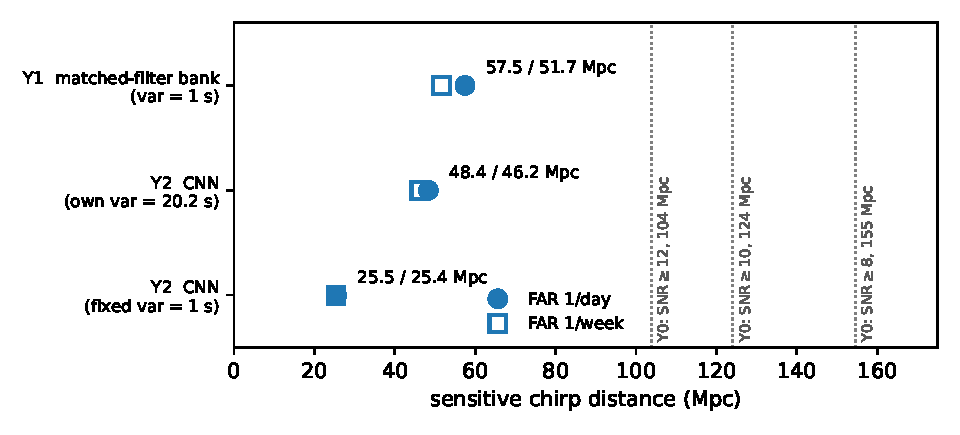
\includegraphics[width=0.85\textwidth]{fig_distances.pdf}
\caption{Sensitive chirp distance of Y1 and Y2 at one false alarm per day (filled) and per week (open), against the
ideal reference Y0 at network SNR 8, 10 and 12 (dotted). Drawn by \texttt{paper/make\_figure.py} from files at the
release tag only.}
\label{fig:dist}
\end{figure}

The distance ratio Y1/Y2, from a paired bootstrap over injections (90\% intervals), is 1.19 (1.10--1.29) at one per
day and 1.12 (1.05--1.20) at one per week when Y2 uses its own tolerance; Y1 finds 111 injections and Y2 96 at one per
day, 93 of them common to both. With both at $\pm1$\,s the ratio is 2.25 (1.86--3.10) and 2.04 (1.69--2.78). The
intervals resample injections only, not the background that sets the thresholds.

So the bank beats the CNN by 12--19\% in distance even when the CNN is allowed its own 20\,s timing tolerance, and
the CNN is not competitive under a tight timing rule because it cannot place a merger to the second. Both reach about
a third of the ideal distance; that gap is the room a better method can take.

\section{Verification}
Every check below is an automated test committed with the release; its output file is named. None is a human review.

\paragraph{Evaluator} (\texttt{golden\_evaluate.py}, synthetic submissions with known answers): a perfect detector
recovers every injection and a sensitive volume within $3\sigma$ of the Monte Carlo truth ($|V - V_{\rm true}| =
9.9\times10^6$ against $3\sigma = 3.8\times10^7\,\mathrm{Mpc}^3$); a blind detector gives zero volume; exactly 27
background triggers lie above the one-per-day threshold; triggers 0.3\,s apart are clustered to the loudest; and a
trigger 30\,s off is found with \texttt{var} 40\,s and not with 20\,s, while \texttt{var} above 60\,s is rejected.
All pass.

\paragraph{Injection path} (\texttt{golden\_injection.py}, against PyCBC): for $0.2+0.2$ and $1+1\,\Msun$ signals in
real strain, the whitened-domain SNR agrees with PyCBC's \texttt{sigma} to $\leq 9\times10^{-10}$ relative; the merger
lands within 0.30\,ms of its expected sample; and a true-template matched filter recovers each injection within 2 of
its optimal SNR. The test used test segment 1249001472 (see Section~\ref{sec:limits}).

\paragraph{Data integrity} (\texttt{verify\_published.py}): GWOSC publishes no checksums, so the 64 saved arrays were
compared with the minimum, maximum, mean and standard deviation that GWOSC's API publishes for each file. Worst
relative error $5.6\times10^{-8}$ (float32 storage); worst mean error $1.05\times10^{-11}$ standard deviations.

\paragraph{Noise spectrum} (\texttt{lowmem\_psd.py}): a numpy re-implementation of the PyCBC PSD estimate used for Y1
and Y2 matches it to $4.7\times10^{-10}$ relative in band, and whitened data to $4.5\times10^{-12}$ absolute (rms 2.29),
with a peak resident memory of 1.02\,GB for the numpy path and 2.10\,GB after also running the PyCBC path.

\paragraph{Y1 pipeline} (\texttt{y1\_bank.py golden}, development segments only): template whitening equals the
reference function exactly; GPU float32 against a float64 reference to $\leq 2.7\times10^{-5}$ relative; windowed
against whole-series filtering to $3.2\times10^{-6}$. The recovery test has a history that belongs in the record. A
first version passed vacuously; a second, which called an injection ``loud'' by chirp distance below 70\,Mpc, failed,
because chirp distance ignores orientation (an injection at $d_c = 58\Mpc$ had optimal SNR 5.9;
\texttt{results/y1\_golden.json}, \texttt{pass: false}). The rule was then changed to optimal network SNR $\geq 10$,
recovered within 1\,s at $\geq 0.7$ of optimal, and tested on two development segments not used before: all 5 loud
injections were recovered at 0.77--0.91 of optimal SNR within 59\,ms (\texttt{y1\_golden\_confirm.json}). This test
was written and run by a separate AI session. It also caught that PyCBC's time-domain TaylorF2 returns 5.000\,s of
samples after coalescence; Y1's templates are cut at coalescence.

\paragraph{Y1 foreground shortcut.} For speed, the foreground is filtered only with the $\pm48$ chirp-mass neighbours
of each injection's own template, while the background uses all 3,235; this can only lower a foreground statistic.
On the 14 held-out development injections the neighbour statistic was 0 to 2.03 below the full-bank one; on the five
loud ones it was equal in four and 0.72 lower in one. Y1 is therefore slightly conservative.

\paragraph{Upstream finding.} During PyCBC waveform generation, resident memory grows with each new waveform length
and is not released (30 random-mass waveforms: about 0.2 to 2.0\,GB; flat when the length repeats). At least part of
it reproduces when calling LALSimulation \cite{lalsuite} directly; whether the library or the system allocator holds
it was not determined, and it was not shown to be unbounded. It is reported as \href{https://github.com/gwastro/pycbc/issues/5554}{gwastro/pycbc\#5554} (open, no reply at
the time of writing) with a standalone reproduction, \texttt{pycbc\_leak\_repro.py}.

\section{Limits}\label{sec:limits}
\begin{itemize}
\item \textbf{Thresholds rest on one background.} The bootstrap intervals do not include threshold uncertainty; the
one-per-week threshold sits on the 4th-loudest background trigger. One per month is not reachable; going deeper needs
more segments or a second slide family.
\item \textbf{Y1 is not the field's best.} Equal-mass templates and an 8-chunk semi-coherent statistic, the strongest
matched filter we could make adequate on one laptop GPU; production searches use far larger banks
\cite{hanna_bank,kacanja_o4a}.
\item \textbf{Y2's timing} was calibrated on 32 development injections; another calibration choice would move its
own-tolerance result but not the $\pm1$\,s one.
\item \textbf{Scope.} Non-spinning TaylorF2, 0.2--1.0\,\Msun, O3a H1 and L1 only, one machine (macOS arm64, Apple
GPU). Results on other platforms are expected to agree to float32 precision, not bit for bit; this was not checked.
Sensitivity to the choice of the 24 test segments beyond the bootstrap was not measured.
\item \textbf{Two uses of a test segment.} The injection-path check and the choice to raise the chirp-distance cap
from 300 to 500\,Mpc used test segment 1249001472. Neither tuned a search statistic, but the release README's rule
``tune nothing on the test segments'' was not followed to the letter.
\end{itemize}

\paragraph{Corrections to the release documentation.} Writing this paper against the committed files found these
discrepancies in the v1.0.0 README, RESULTS and PLAN; the numbers in this paper follow the files.
(i)~The README calls the Y1 recovery rule ``fixed before the test''; that holds only for the confirmation run, after the
failed first rule described above, which the README does not mention. Under the final rule, the first two development
segments give a lowest recovery of 0.76, slightly below the ``$\geq 0.77$'' quoted.
(ii)~``Windowed within $3\times10^{-6}$'' should read $3.2\times10^{-6}$; ``GPU within $3.5\times10^{-5}$'' is from a
coarse smoke run, and the full runs give $2.7\times10^{-5}$.
(iii)~The Y1/Y2 bootstrap output is committed, but the script that produced it is not, and the file does not record
the resample count (2,000 per RESULTS). The original script and its random seed were not preserved. Version 1.0.1 adds a
script rebuilt from the documented design. Its seed and the order in which it draws for the four comparisons were
recovered by search over seeds 0--499 and all 24 orders: exactly one combination reproduces all four intervals, and
the committed file, byte for byte.
(iv)~The PLAN promised an efficiency curve against optimal SNR; the evaluator does not produce one. The PLAN's
``download about 3\,GB'' is stale (8.3\,GB).
(v)~The README's ``PSD estimate adds about 1.6\,GB per segment'' comes from a different measurement from the committed
check, which shows 1.08\,GB between the two paths.

\section{Reproducibility}
Environment of the published numbers: macOS 27.2 on arm64 with the Apple GPU, Python 3.12.13, numpy 2.4.6, scipy
1.17.1, torch 2.12.0, PyCBC 2.10.0 \cite{pycbc_soft}, gwpy 4.0.1, LAL 7.7.1; the exact package set is
\texttt{primordial\_blackhole\_search/requirements-lock.txt}. From a clean checkout of tag \texttt{longchirp-v1.0.1}
\cite{deepstrain101} (results identical to v1.0.0): build the environment, fetch the data (about 8.3\,GB downloaded one
file at a time, about 4.1\,GB kept), then run \texttt{golden\_evaluate.py}, \texttt{golden\_injection.py} and
\texttt{evaluate.py} on a submission; \texttt{bootstrap\_y1\_y2.py --check} reproduces the ratio intervals. Y2's submission is
committed; Y1's is regenerated from the committed per-segment maxima. Recorded run times: Y1 background 28.3\,h
(3,235 templates over 24 segments), Y1 foreground about 4.5\,h. A claim-by-claim guide with expected outputs is in
\texttt{paper/REFEREE\_GUIDE.md}.

\section{AI assistance}
This work was done by one independent author with substantial help from Anthropic's Claude models (several
versions). The models wrote most of the code, ran most of the analyses and drafted this paper; the author chose the
questions, directed and reviewed the work, and takes responsibility for its content. The checks reported here are
automated tests and comparisons with independent references (PyCBC, GWOSC's published statistics), plus a test run
by a separate AI session. They are not human peer review, and no external expert has read this work yet.

\paragraph{Acknowledgement.} This research has made use of data or software obtained from the Gravitational Wave Open
Science Center (gwosc.org), a service of the LIGO Scientific Collaboration, the Virgo Collaboration, and KAGRA. This
material is based upon work supported by NSF's LIGO Laboratory which is a major facility fully funded by the National
Science Foundation, as well as the Science and Technology Facilities Council (STFC) of the United Kingdom, the
Max-Planck-Society (MPS), and the State of Niedersachsen/Germany for support of the construction of Advanced LIGO and
construction and operation of the GEO600 detector. Additional support for Advanced LIGO was provided by the
Australian Research Council. Virgo is funded, through the European Gravitational Observatory (EGO), by the French
Centre National de Recherche Scientifique (CNRS), the Italian Istituto Nazionale di Fisica Nucleare (INFN) and the
Dutch Nikhef, with contributions by institutions from Belgium, Germany, Greece, Hungary, Ireland, Japan, Monaco,
Poland, Portugal, Spain. KAGRA is supported by Ministry of Education, Culture, Sports, Science and Technology (MEXT),
Japan Society for the Promotion of Science (JSPS) in Japan; National Research Foundation (NRF) and Ministry of Science
and ICT (MSIT) in Korea; Academia Sinica (AS) and National Science and Technology Council (NSTC) in Taiwan.

\begin{thebibliography}{99}\small
\bibitem{carr2020} B. Carr and F. K\"uhnel, Primordial black holes as dark matter: recent developments,
Annu. Rev. Nucl. Part. Sci. 70, 355 (2020), \href{https://doi.org/10.1146/annurev-nucl-050520-125911}{doi:10.1146/annurev-nucl-050520-125911}.
\bibitem{lvk_o3a_ssm} R. Abbott et al. (LIGO Scientific, Virgo and KAGRA Collaborations), Search for subsolar-mass
binaries in the first half of Advanced LIGO's and Advanced Virgo's third observing run, Phys. Rev. Lett. 129, 061104
(2022), \href{https://doi.org/10.1103/PhysRevLett.129.061104}{doi:10.1103/PhysRevLett.129.061104}.
\bibitem{lvk_o3b_ssm} LIGO Scientific, Virgo and KAGRA Collaborations, Search for subsolar-mass black hole binaries in
the second part of Advanced LIGO's and Advanced Virgo's third observing run, Mon. Not. R. Astron. Soc. 524, 5984
(2023), \href{https://doi.org/10.1093/mnras/stad588}{doi:10.1093/mnras/stad588}; correction
\href{https://doi.org/10.1093/mnras/stad3120}{doi:10.1093/mnras/stad3120}.
\bibitem{nitz_wang_o3a} A. H. Nitz and Y.-F. Wang, Search for gravitational waves from the coalescence of sub-solar
mass binaries in the first half of Advanced LIGO and Virgo's third observing run, Phys. Rev. Lett. 127, 151101 (2021),
\href{https://doi.org/10.1103/PhysRevLett.127.151101}{doi:10.1103/PhysRevLett.127.151101}.
\bibitem{kacanja_o4a} K. Kacanja et al., Search for sub-solar mass binaries in the first part of LIGO's fourth
observing run, \href{https://arxiv.org/abs/2602.12115}{arXiv:2602.12115}.
\bibitem{hanna_bank} C. Hanna et al., Template bank for sub solar mass compact binary mergers in the fourth observing
run of Advanced LIGO, Advanced Virgo, and KAGRA, \href{https://arxiv.org/abs/2412.10951}{arXiv:2412.10951}.
\bibitem{gabbard2018} H. Gabbard, M. Williams, F. Hayes and C. Messenger, Matching matched filtering with deep networks
for gravitational-wave astronomy, Phys. Rev. Lett. 120, 141103 (2018),
\href{https://doi.org/10.1103/PhysRevLett.120.141103}{doi:10.1103/PhysRevLett.120.141103}.
\bibitem{george2018} D. George and E. A. Huerta, Deep neural networks to enable real-time multimessenger
astrophysics, Phys. Rev. D 97, 044039 (2018), \href{https://doi.org/10.1103/PhysRevD.97.044039}{doi:10.1103/PhysRevD.97.044039}.
\bibitem{mlgwsc1} M. B. Sch\"afer et al., First machine learning gravitational-wave search mock data challenge,
Phys. Rev. D 107, 023021 (2023), \href{https://doi.org/10.1103/PhysRevD.107.023021}{doi:10.1103/PhysRevD.107.023021}.
\bibitem{deepstrain} S. Pal, DeepStrain: deep-learning searches of public LIGO/Virgo data for black-hole signatures,
version longchirp-v1.0.0, Zenodo (2026), \href{https://doi.org/10.5281/zenodo.24399603}{doi:10.5281/zenodo.24399603}.
\bibitem{deepstrain101} S. Pal, DeepStrain, version longchirp-v1.0.1, Zenodo (2026), DOI to be added when minted.
\bibitem{gwosc_o3} R. Abbott et al. (LIGO Scientific, Virgo and KAGRA Collaborations), Open data from the third
observing run of LIGO, Virgo, KAGRA, and GEO, Astrophys. J. Suppl. Ser. 267, 29 (2023),
\href{https://doi.org/10.3847/1538-4365/acdc9f}{doi:10.3847/1538-4365/acdc9f}.
\bibitem{buonanno2009} A. Buonanno, B. R. Iyer, E. Ochsner, Y. Pan and B. S. Sathyaprakash, Comparison of
post-Newtonian templates for compact binary inspiral signals in gravitational-wave detectors, Phys. Rev. D 80, 084043
(2009), \href{https://doi.org/10.1103/PhysRevD.80.084043}{doi:10.1103/PhysRevD.80.084043}.
\bibitem{allen2005} B. Allen, A $\chi^2$ time-frequency discriminator for gravitational wave detection, Phys. Rev. D
71, 062001 (2005), \href{https://doi.org/10.1103/PhysRevD.71.062001}{doi:10.1103/PhysRevD.71.062001}.
\bibitem{babak2013} S. Babak et al., Searching for gravitational waves from binary coalescence, Phys. Rev. D 87,
024033 (2013), \href{https://doi.org/10.1103/PhysRevD.87.024033}{doi:10.1103/PhysRevD.87.024033}.
\bibitem{pycbc_usman} S. A. Usman et al., The PyCBC search for gravitational waves from compact binary coalescence,
Class. Quantum Grav. 33, 215004 (2016), \href{https://doi.org/10.1088/0264-9381/33/21/215004}{doi:10.1088/0264-9381/33/21/215004}.
\bibitem{pycbc_soft} A. Nitz et al., PyCBC (software), Zenodo, \href{https://doi.org/10.5281/zenodo.596388}{doi:10.5281/zenodo.596388}
(version 2.10.0 used here).
\bibitem{lalsuite} LIGO Scientific Collaboration, LIGO Algorithm Library (LALSuite), \href{https://doi.org/10.7935/GT1W-FZ16}{doi:10.7935/GT1W-FZ16}.
\end{thebibliography}
\end{document}
